\documentclass[a4paper, twosided, openany]{memoir}
\usepackage{hyperref}
\hypersetup{
  colorlinks,
    linkcolor={black},
    citecolor={black},
    urlcolor={blue}
}
\usepackage{graphicx}

\setlrmarginsandblock{3cm}{2.5cm}{*}
\setulmarginsandblock{2.5cm}{2.5cm}{*}
\checkandfixthelayout
\setlength{\evensidemargin}{\oddsidemargin}

\begin{document}

\pagestyle{plain}
\chapterstyle{demo3}
\title{Advanced HTML XBlock for Open EdX platform}
\date{\today}

\frontmatter

\maketitle

\pagebreak

\begin{abstract}
The project focuses on enhancing the open edx html component. Current html component does not
allow a fully fledged html, css and javascript content to be added in course. Also the html editor of
the current component is not very user friendly and lacks some fundamental functionalities such as
code indentation, code folding etc. Our first approaach was to modify openedx system itself and
thus changing the html editor for all users. Lateron we decided to move to devloping an xblock for
this and hence making it optional. We also added extra features to enahance the functionality of
xblock. These extra features include live previewing the html content along with editor.
\end{abstract}

\pagebreak

\renewcommand{\abstractname}{Acknowledgements}
\begin{abstract}
	We, the summer interns of this group, are overwhelmed in all humbleness and
gratefulness to acknowledge our deep gratitude to all those who have helped us put
our ideas to perfection and have assigned tasks well above the level of simplicity and
into something concrete and unique.
We, wholeheartedly thank Prof. D.B. Phatak for having faith in us, selecting us to be
a part of his valuable project and for constantly motivating us to do better.
We thank Miss Kalpana Kannan for providing us the opportunity to work on this
project.We are also very thankful to our mentors Mr. Hitesh Murkute and Mr. Sachin R Shirsat
for their valuable suggestions. They were always there to show us the right track when needed help.
With help of their brilliant guidance and encouragement, we all were able to complete
our tasks properly and were up to the mark in all the tasks assigned. During the
process, we got a chance to see the stronger side of our technical and nontechnical
aspects and also strengthen our concepts.
Last but not the least, we wholeheartedly thank all our other colleagues working in
different projects under Prof. D.B Phatak for helping us evolve better with their critical advice.
\end{abstract}

\pagebreak

\tableofcontents

\mainmatter

\chapter{Introduction}

Open edX is a widely used and very popular MOOC platform. The Open edX software is a opensource
technology that makes learning easier and studying faster. It was created by MIT and
Harvard University, and was quick to gain support of universities such as UC Berkely, Georgetown,
and Stanford.
The software platform is designed to engage students and teachers in an interactive, modular way. It
promotes active learning by video snippets, interactive components and game-like experience. The
course content is presented through learning sequences: a set of interwoven videos, readings,
discussions, wikis, collaborative and social media tools, exercises and materials with automatic
assessments and instant feedback.
The Open edX project is a global success. It powers major MOOC initiatives, hosting blended and
online courses, all around the world.
\chapter{Getting started}
\section{Limitations of the present HTML editor in OpenEdx}
Open edX in itself is a humongous learning management system with unparalleled feature list. It is
among the top MOOCs platforms in the world. As it is the way of the world, there is nothing perfect
here and Open edX is not an exception. All applications/platforms have a scope to enhance its
features and abilities of its components. In this project we worked on enhancing the HTML
component which is used for content creation in courses.\newline\newline
While current HTML editor does the job well but it has got its own mind and behaves with
uncertainty sometimes. Enhancing the editor with internal CSS and ironing out the indentation
issues will boost the user experience of the course creator. Our aim was to develop and integrate a
full-fledged HTML editor like Notepad++ or Sublime for Open edX.\newline\newline
Here are some issues that we have encountered in the HTML editor used by the OpenEdx platform
\begin{enumerate}
  \item \textbf{Indentaion in the current HTML editor :-}\newline\newline
The purpose of code indentation and style is to make the program more readable and
understandable. It saves lots of time while we revisit the code and use it.
Code indentaion in an important part towards increasing the aesthetic of any editor,
as it increases readability and makes understanding of the code easier.\newline\newline
In Open edX however the code indentation feature is not implemented in the raw
HTML editor, which is the CodeMirror v3.21.0. This is mainly because the version
of CodeMirror used in Open edX has been implemented with a minimalistic use case
and has not been updated since October 2015. The problem is that even if we
manually indent our code, once we save our progress and close the raw editor, the
indentation is lost i.e it doesn’t gets saved. 

  \item \textbf{Code Folding in the current HTML editor :-}\newline\newline
Code folding is a feature of some text editors, source code editors, and IDEs that
allows the user to selectively hide and display – "fold" – sections of a currently edited
file as a part of routine edit operations. This allows the user to manage large
amounts of text while viewing only those subsections of the text that are specifically
relevant at any given time.\newline\newline
This is a pretty useful feature for any editor and presents the user with various use
patterns, primarily organizing code or hiding less useful information so one can
focus on more important information. Since the CodeMirror version implemented in
Open edX is very old this feature is not available and thus was added to our List of
possible enhancements.

  \item \textbf{Internal CSS in HTML Code :-}\newline\newline
Cascading Style Sheets (CSS) is a style sheet language used for describing the
presentation of a document written in a markup language like HTML CSS is a
cornerstone technology of the World Wide Web alongside HTML and JavaScript.\newline\newline
The three main types of CSS styles are inline, internal and external. Currently in
Open edX platform in the raw HTML editor only inline or embedded CSS support is
available. Inline styles are CSS styles that are applied directly in the page's HTML.
Because inline styles they are the most specific in the cascade, they can over-ride
things we didn't intend them to. They also negate one of the most powerful aspects
of CSS - the ability to style lots and lots of web pages from one central CSS file to
make future updates and style changes much easier to manage.\newline\newline
If we had to only use inline styles, our documents would quickly become bloated and
very hard to maintain. This is because inline styles must be applied to every element
we want them on. That is why internal CSS is preferred whenever exhaustive use of
CSS is required as opposed to inline CSS. Internal CSS is Open edx raw HTML
editor is not supported as internal CSS must be defined inside the style tag in the
head element of the html body. However the raw HTML editor of Open edX stips
down style tags and the effects are not reflected as wanted. Styles of other
components in the web page also gets changed which we do not want. Thus allowing
internal CSS is an important enhancement criterion which should be addressed.
\end{enumerate}

To understand the limitations better we have provided the screenshots as mentioned
below:
\begin{center}\textbf{[See Figures 1-4 in the “Figures and Screenshots” section.]}\end{center}


\section{Objectives}
Here are the list of enhancements we were aiming for in the html component of Open edX:
\begin{itemize}
  \item Improvise the raw HTML editor to have features like pretty indentation, code folding
etc.
  \item Check if we can add a separate CSS section in raw HTML editor to eliminate inline
CSS
\item Fix the cursor placement issue and some other minor issues.
\end{itemize}

\section{Observations}
Regarding the Open edX paltform and the editors used in the Open Edx one might come up with thefollowing kind of questions
\begin{itemize}
\item Is OpenEdx using a raw editor or visual editor or both ?
\item Did OpenEdx write their own editor ?
\item If yes, then what how is it working ?
\item If no, then from where they have implemented their text editors
\item What kind of editor are they using ?
\item Where do we find the editors source code ?
\item How many editors are they using ?
\item Their method of working ?
\item Their current scenario ?
\item On what basis is this editor working along with the OpenEdx platform ?\newline\newline
\end{itemize}


To all these queries here are some facts that would be helpful:
\begin{enumerate}
\item OpenEdx uses both the visual editor as well as the raw editor.
\item OpenEdx has not written their own editor neither the visual editor nor the raw editor.
\item OpenEdx uses open source text editors for this purpose.
\item The visual editor is tinyMCE editor and the raw editor is CodeMirror Editor.
\item These editors are located in edx source code, in github.
\item CodeMirror is made to work in the custom mode configuration. OpenEdx is using a very old version of CodeMirror.
\item The tinymce editor folder of openedx consists of a plugin called "codemirror-for-tinymce".
\item The good thing about this plugin is that any version of codemirror can be used in the code and it will work perfectly fine.
\item The “codemirror-for-tinymce” plugin is already in use in the OpenEdx repository.
\item We can use the “codemirror-for-tinymce” plugin for tinymce 4.x.x versions.
\item There is an xblock module or simply an xblock called html-module.py
\item This particular xblock module handles the operation of the html editor.
\item This is the module that loads the html editor widget and configures both (tinymce and codemirror) editors to work hand in hand with the help of “codemirror” plugin for tinymce.
\end{enumerate}


\section{Our plan of action}

Depending on the facts that we uncovered regarding the html editors we have come up with
two possible approaches initially, that would fulfill our required objectives.
\begin{enumerate}

\item\textbf{Approach I}\newline Updating the present version of WYSIWYG and raw HTML editors in Open
edX
\item\textbf{Approach II}\newline Integrating other third party open source text editors into OpenEdx platform.
\end{enumerate}

%%%%%%%%%%%%%%%%%%%%%%%%%%%%%%%%%%%%%%%%%%%%%%%%%%%%%%%%%%%%%%%%%%%%%%%%%

\chapter{Approach I - Local integration}
\section{Updating the present version of Editors present in Open edX}
Our first approach was to download the latest versions of TinyMCE, CodeMirror and
the plugin “codemirror-for-tinymce” from their respective git repositories into our local
Machine.\newline
Next step was to integrate the two editors i.e., CodeMirror and TinyMCE using the plugin and
test it on our local machine, and later integrate it with Open edX using one of the Open edX developing
environment.\newline
The result would be TinyMCE loading the instance of latest version of CodeMirror as its
raw HTML editor.
However this implementation could only solve the indentation and code folding problem,
but still the internal css problem wouldn’t be solved just with this.\newline\newline
For enabling the internal CSS we thought of two possible implementations:
\begin{enumerate}
\item\textbf{Using Iframes}\newline
For this, we were planning to wrap the entire html content inside an iframe
and then add theming to the iframe.
\begin{itemize}
\item Set the width of iframe to 100\%
\item Set the height of iframe equal to the height of content of iframe
\item Set the border of iframe to zero/none
\item Open all hyperlinks within the iframe in new tab
\end{itemize}
Hence the expected result is an invisible iframe holding our HTML content.



\item\textbf{Using JavaScript}\newline
This is a slightly tough and critical approach, which was to apply CSS using
JavaScript. The plan was to separate out CSS part from HTML content and
wrap the entire content in a html div tag with an unique id.
Next we would have to manually select each and every child of the div by
parsing the DOM (Document Object Model) tree and apply styles to it.\newline
\end{enumerate}

We opted for the first i.e the Iframe approach because of the following reasons:
\begin{enumerate}
\item This method allows the course content creator to include third party CSS such as
bootstrap, w3css which will make the course even more beautiful
\item Implementaion is easier
\item Wrapping data inside the iframes containerizes the data ensuring no mixing of
CSS between two HTML blocks in LMS.
\item The overhead of the second approach will be very large, since parsing
the DOM tree would take considerable amount of time and effort.
\end{enumerate}


\section{Implementation of our Local integration}
In the first phase of implementing our approach of updating the present editors, we
first downloaded both the editors onto our local machine and then integrated the latest
version of CodeMirror and TinyMCE in our local machine. Later we integrated it with
Django framework since Open edX uses Django framework in the back end as their Web
Application Framework. This step was done to give us a better insight into the interaction of
the present editors in Open edX with Django. The steps of our implementation are
mentioned in brief below:
\begin{enumerate}
\item Firstly, we had downloaded the latest version of CodeMirror and TinyMCE from their
github repositores and then tested them individually to check whether all the desired features
are working or not.
\item Secondly, we had downloaded the latest version of the “codemirror-for-tinymce” plugin
from its git repo.
\item Next we had replaced the default raw HTML editor of TinyMCE with our instance of the
latest version of CodeMirror. This was done by configuring the \textbf{init-tinymce.js} file to use
CodeMirror as an external plugin and thus load it as its default raw HTML editor.
\item Later, for enabling the internal CSS we had encapsulated the entire html content of the
editor into an iframe.
\item We have then set the width of the iframe to 100 percent and set the height of the iframe
equal to the height of the html content.
\item  We had made sure that the borders of iframe was set to zero to make it invisible so that
the user experience is better and smooth.
\item After completing our stand alone integration we merged it with a Django project to run
our editor as an app in the Django server. This integration was quite useful as Open edX
itself uses Django framework in its backend and it helped us in understanding about the
Django back end of Open edX.
\end{enumerate}


\section{Summary of our local integration}
After completing our local integration, firstly we had tested our local instances of
TinyMCE and CodeMirror on the Django server. A brief summary of our observations are
listed below.
\begin{enumerate}
\item Most of the HTML tags and their atrributes are working fine. Some of the exceptions
being script tag , audio tag etc.
\item Almost every CSS style and attributes work fine. The exceptions are those style features
which by default require a script tag to be implemented.
\item CSS animations can be implemented and other third party HTML-and CSS-based design
templates such as Bootstrap can be linked and used without any error.
\item We prepared a detailed Test Report which can be found here:\newline[\url{https://docs.google.com/spreadsheets/d/1AJQWfAG2NIjpxFZt2fnLPlKdhP2-q35KZ0DOmdb-F0w/edit#gid=0}]
\item  Source code is available in our github repository here:\newline[\url{https://github.com/ashutoshbsathe/codemirror-in-tinymce}]
\end{enumerate}


\section{Issues faced and solutions}
\begin{enumerate}

\item\textbf{AJAX:}\newline\newline
We had no idea about how to pass data between RESTful APIs at first. Then later we
found out that this can be done via a request called as AJAX which basically passes
the data in JSON format from one API to another API. And hence we used the same.
On a button click in our html, we would send the AJAX query from webpage to
Django backend. While this seems easy at first, it is a bit tricky when we are using
only a single text area and not entire form element. So the main problem was our
csrf\_token was not being set correctly since we were not using a form. So we
decided to completely skip the csrf authentication by adding @csrf\_exempt
decorator to our view

\item\textbf{Stripping of style tags:}\newline\newline
So tinyMCE does not allow you to directly add CSS in your html. It will constantly
filter out your own \verb=<style>= and \verb=<link>= tags out of it’s display content. The only way
to get around this is by setting valid\_children, valid\_elements and
extended\_valid\_elements properly in TinyMCE config.

\item\textbf{Indentation in the “CodeMirror with TinyMCE setup” :}\newline\newline
Now because the tinymce keeps filtering out content, there’s no actual way to show a
nice indented code in CodeMirror. For this we found a script that will indent our
html code nicely and we called it before setting the content in CodeMirror. One thing
to note here is that whatever indentation that was done in CodeMirror was a bit of a
pseudo Indentation and not true indentation as the course creator wants. Sure, it was
nicely indented, but if somewhere content creator specifically wanted a specific tag
on multiple line such as
\begin{verbatim}
<a href=”https://www.google.com”>
A SearchEngine
</a>
\end{verbatim}
It won’t be rendered in that way because the script treats anchor tag as a single-line
tag and it will be rendered as follows:
\begin{verbatim}
<a href=”https://www.google.com”>ASearchEngine</a>
\end{verbatim}
Sadly enough, there is no way for tinyMCE to shut down it’s content filtering and
hence this issue remains unsolved.


\item\textbf{Unnecessary modification of html code:}\newline\newline
This issue specifically occurs when you try to edit something that was added in raw
mode. For example, let’s hope you add a nice CSS animation and then return back to
tinyMCE for saving the content, while returning back, you accidently clicked in the
div of your animation and you pressed enter. Then tinymce will try to split your div
in half breaking it where you pressed enter, and will also add some bad html code
which you definitely don’t want. Again this issue is unavoidable because of content
filtering algorithms used in tinyMCE.
\end{enumerate}

%%%%%%%%%%%%%%%%%%%%%%%%%%%%%%%%%%%%%%%%%%%%%%%5

\chapter{Approach I- Open edX intregation}
After testing our hybrid local intregation, and setting up our developing environment for Open edX,
the next phase was to integrate it with the running instance of Open edX on our Devstack
\section{Plan of action}
The idea and plan behind intregating our running hybrid instance of CodeMirror in TinyMCE with
Open edX is mentioned below:
\begin{enumerate}
\item\textbf{Indentation and code folding features}
\begin{itemize}
\item Add the latest version of CodeMirror v5.38.0 to the source code of Open edX
leaving the older version untouched.
\item Configure TinyMCE to open the updated version of CodeMirror as its raw HTML
editor.
\item Test the updated CodeMirror in TinyMCE and see if its wroking as expected.
\end{itemize}
\item\textbf{Enabling internal CSS}
\begin{itemize}
\item Understand the working of the XModule html\_module.py which is the widget
which loads the WYSIWYG editor in Open edX.
\item Learn how the html content is getting stored in the MongoDB .
\item The idea was to wrap the html content inside an inframe before it gets stored in the
Database. However this was to be done only when the course authors used internal
CSS in thier courses.
\item Similarly, while loading the content in LMS, it would be wrapped inside and iframe
first and then rendered in order to produce the desired effect.
\end{itemize}
\end{enumerate}

\section{Implementation}
\subsection{Configuring TinyMCE to use updated CodeMirror v5.38.0}
\begin{itemize}
\item The CodeMirror and TinyMCE source files are located in the edx-platfrom can be found on
the following path : \textit{\textbf{edx-platform/common/statis/js/vendor}}
\item Inside the tinymce source code, we placed the updated version of CodeMirror in the plugins
folder for TinyMCE.\newline The path was :
\textit{\textbf{edx-platform/common/static/js/vendor/tinymce/js/tinymce/plugins}}
\item Next we configured TinyMCE to use the updated CodeMirror as its raw HTML editor. This
was done through making changes in the TinyMCE configuration file \textbf{edit.js} located here :\newline
\textbf{\textit{edx-platform/common/lib/xmodule/xmodule/js/src/html/edit.js}}
\item Similarly, while loading the content in LMS, it would be wrapped inside and iframe
first and then rendered in order to produce the desired effect.
\end{itemize}
After performing the following steps we were able to configure TinyMCE to open our updated
instance of CodeMirror v5.38.0 as its raw HTML editor succesfully. Features such as indentation,
code-folding etc were working fine

\subsection{Using Iframes to enable internal CSS}
\subsubsection{Issues faced}
Once we were able to intreagte updated version of CodeMirror with TinyMCE, we tried testing
internal CSS in our new editor. Our observations are mentioned below:
\begin{itemize}
\item  The effect of the internal CSS is only visible inside the WYSIWYG editor i.e inside
TinyMCE.
\item  Once we save our progress the Open edX backend automatically strips the style tag and
removes it. As a result of this, no effect of the CSS is visible in the actual course content.
\end{itemize}

\section{Change in Approach}
\subsection{What happened to the issues}
We tried to look into the issues by looking into openedx backend by logging at several places in
several different xmodules and we failed. We discussed this issue with Aparna Ma’am(Mentor,
IITBombayX team). She said that we were on a right track and we should play with backend
through logs itself. Strangely enough, there were NO logs generated at all!! This lead us to a
roadblock situation where we need to switch to another approach for checking out backend.
However, all of the ways went at least once through logging step which was not working on our
devstack very well. We also discovered that the server provided to us for R\&D
purposes(10.129.27.44) also was unable to generate any logs.
\subsection{Need for change in approach}
Because of these issues, we were facing a major roadblock ahead of us and hence we need to
switch approaches. Now we had 2 more options, Xblock and integrating entirely a new editor into
an already complex openedx system which does not even generate logs ! Another option was to
reinstall devstack and see what causes devstack to not generate logs. But the clock was ticking and
we only hand 2.5 weeks left for the internship period. We could have pursued approach 1 to the end
and maybe end the internship without completing the project but we chose to change approach.
\subsection{Why Xblock approach and not integrating editors such as
contenttools/grapejs ?}
Two main reasons:
\begin{enumerate}
\item If we wanted to integrate any of these with OpenEdx, we would need the logger to be working
perfectly. And as described in the issues above, that is what kept us from pursuing approach 1 itself
\item Xblocks are modular. If we decide to modify the system, we’re forcing the editor changes to all
users. And probably some of these users don’t even need this advanced editor and features. On the
other hand, if we make this into an xblock, it will be used by people who actually need it and know
how to use it. Also one hidden advantage of xblock is that they are largely platform independent.
Most of the xblocks do not need to be updated on every single version of openedx since the core
Xblock API remains unchanged.
\end{enumerate}
%%%%%%%%%%%%%%%%%%%%%%%%%%%%%%%%%%%%%%%%%%%%%%%%%


\chapter{Basics of developing an XBlock}
\section{Introduction}
XBlock is a way to create rich engaging courses. XBlock is a component architecture of edX, and a
course can be build from the different Blocks as pieces. On the other hand, XBlock will offer
APIs and structure for other modules in the edX to comunicate with the course content since all
other web applications in a online ecosystem needs to access the course content.\newline
XBlock is the software development kit for edX-MOOC and it is written in python2. XBlock
generally contains few python classes which create a small web application. So, to create new
xblocks, a new module called xblock-sdk has been open sourced. Creating a new xblock means
creating a simple python installable python package with a class derived from the XBlock.

\section{XBlock API and Runtimes}
Any web application can be an XBlock runtime by implementing the XBlock API. The
XBlock API is not a RESTful API. XBlock runtimes can compose web pages out of XBlocks that
were developed by programmers who do not need to know anything about the other components
that a web page might be using or displaying.

\section{XBlocks for Developers}
Developers can select from functionality developed by the Open edX community by installing an
XBlock on their instance of Open edX. Developers can integrate new or propriety functionality for
use in XBlock runtimes by developing a new XBlock using the supported XBlock API.\newline\newline
XBlocks are like miniature web applications: they maintain state in a storage layer, render
themselves through views, and process user actions through handlers. XBlocks differ from web
applications in that they render only a small piece of a complete web page. Like HTML \verb=<div>= tags,
XBlocks can represent components as small as a paragraph of text, a video, or a multiple choice
input field, or as large as a section, a chapter, or an entire course.
\section{Criteria}
One must design a XBlock to meet two criteria:-
\begin{itemize}
\item The XBlock must be independent of other XBlocks. Course teams must be able to use the
XBlock without using other Xblocks.
\item The XBlock must work together with other XBlocks. Course teams must be able to combine
different XBlocks in flexible ways.
\end{itemize}

\section{Building an Xblock}
\subsection{Instalingl XBlock Prerequisites}
To build an XBlock, we must have the following tools on our computer.
\begin{itemize}
\item Python 2.7
\item Git
\item A Virtual Environment
\end{itemize}
\subsubsection{Python 2.7}
To run the a virtual environment and the XBlock SDK, and to build an XBlock, we must
have Python 2.7 installed on our computer.
\subsubsection{Git}
EdX repositories, including XBlock and the XBlock SDK, are stored on GitHub. To build
our own XBlock, and to deploy it later, we must use Git for source control.
\subsubsection{A Virtual Environment}
It is recommended that we develop our XBlock using a Python virtual environment. A
virtual environment is a tool to keep the dependencies required by different projects in
separate places. With a virtual environment we can manage the requirements of our XBlock
in a separate location so they do not conflict with requirements of other Python applications
we might need.

\subsection{Setting Up the XBlock Software Development Kit}
After installing all prerequisites, we are ready to set up the XBlock SDK in a virtual environment.
To do this, we must complete the following steps.
\begin{itemize}
\item Create a Directory for XBlock Work
\item Create and Activate the Virtual Environment
\item Clone the XBlock Software Development Kit
\end{itemize}
\subsubsection{Creating a Directory for XBlock Work}
It is recommended that we create a directory in to store all our XBlock work, including a
virtual environment, the XBlock SDK, and the XBlocks we develop.
\begin{enumerate}
\item At the command prompt,we can run the following command to create the directory.
\begin{center}\verb=$ mkdir xblock_development=\end{center}
\item Change directories to the xblock\_development directory.
\begin{center}\verb=$ cd xblock_development=\end{center}
\end{enumerate}
The rest of our work will be from this directory.

\subsubsection{Creating and activating an Virtual Environment}
We must have a virtual environment tool installed on our computer. Then we can create the virtual
environment in our xblock\_development directory.
\begin{enumerate}
\item At the command prompt in xblock\_development,we can run the following command to
create the virtual environment.
\begin{center}\verb=$ virtualenv venv=\end{center}
\item Next Run the following command to activate the virtual environment.
\begin{center}\verb=$ source venv/bin/activate=\end{center}
\item When the virtual environment is activated, the command prompt shows the name of
the virtual directory in parentheses.
\begin{center}\verb= (venv) $=\end{center}
\end{enumerate}


\subsubsection{Cloning the XBlock Software Development kit}
The XBlock SDK is a Python application that helps us build new XBlocks. The XBlock
SDK contains three main components:
\begin{enumerate}
\item An XBlock creation tool that builds the skeleton of a new XBlock.
\item An XBlock runtime for viewing and testing our XBlocks during development.
\item Sample XBlocks that we can use as the starting point for new XBlocks, and for our
own learning.
\end{enumerate}
After we create and activate the virtual environment, we must clone the XBlock SDK and
install its requirements. To do this,we must complete the following steps at a command prompt.
\begin{enumerate}
\item In the xblock\_development directory,we must run the following command to clone the
XBlock SDK repository from GitHub.
\begin{center}\verb=(venv) $ git clone https://github.com/edx/xblock-sdk.git=\end{center}
\item Next Run the following command to change to the xblock-sdk directory.
\begin{center}\verb=(venv) $ cd xblock-sdk=\end{center}
\item Run the following command to install the XBlock SDK requirements.
\begin{center}\verb=(venv) $ pip install -r requirements/base.txt=\end{center}
\item Run the following command to return to the xblock\_development directory,
where we will perform the rest of our work.
\begin{center}\verb=(venv) $ cd ..=\end{center}
\end{enumerate}
When the requirements are installed, we are in the xblock\_development directory, which
contains the venv and xblock-sdk subdirectories. We can now create our Xblock.


\subsection{Creating an Xblock}
Before we can continue,we must make sure that we have set up the XBlock SDK. We then create the XBlock
and deploy it in the XBlock SDK.
\begin{itemize}
\item Create an XBlock
\item Install the XBlock
\item Create the SQLite Database
\item Run the XBlock SDK Server
\end{itemize}

\subsubsection{Creating an XBlock}
We use the XBlock SDK to create skeleton files for an XBlock. To do this,we can follow
these steps at a command prompt.
\begin{enumerate}
\item Change to the xblock\_development directory, which contains the venv and xblocksdk
subdirectories.
\item Run the following command to create the skeleton files for the XBlock.
\begin{center}\verb=(venv) $ xblock-sdk/bin/workbench-make-xblock=\end{center}
\item At the command prompt, we must enter the Short Name we selected for our XBlock.
\begin{center}\verb=$ Short name: myxblock=\end{center}
\item At the command prompt,we must enter the Class name we selected for our XBlock.
\begin{center}\verb=$ Class name: MyXBlock=\end{center}
\end{enumerate}
The skeleton files for the XBlock are created in the myxblock directory

\subsubsection{Installing the Xblock}

After we create the XBlock, we can install it in the XBlock SDK.
In the xblock\_development directory,we can use pip to install our XBlock.
\begin{center}\verb=(venv) $ pip install -e myxblock=\end{center}
We can then test our XBlock in the XBlock SDK

\subsubsection{Running the XBlock SDK Server}
To see the web interface of the XBlock SDK, we must run the SDK server.
In the xblock\_development directory, we can run the following command to start
the server.
\begin{center}\verb=(venv) $ python xblock-sdk/manage.py runserver=\end{center}

\subsubsection{Getting Help for the XBlock SDK Server}
To get help for the XBlock SDK runserver command, we can run the following
command.
\begin{center}\verb=(venv) $ python xblock-sdk/manage.py help=\end{center}
The command window lists and describes the available commands.



\section{Customizing our XBlock}
\begin{enumerate}
\item \textbf{Define Fields:}\newline
The first step in this process is defining field, so, the data of these field types will be
stored by the xblock.
\item\textbf{ Define Views:}\newline
The Views are needed to create HTML pages to display blocks in the course page. It
is simple to render html pages but its difficult to show what we want on the course
page. The view also takes the help of CSS and JavaScript to help the html pages.
\item \textbf{Define Handlers:}\newline
When course web pages are interactive, we will get events from the Javascript to
handle. So, handler is a function to respond to a specific URL. Here we can use the
URL to comumicate with the server too.
\end{enumerate}


%\section{Rendering courseware using XBlocks}
%\subsection{Sequence diagram}

\begin{figure}[!]
	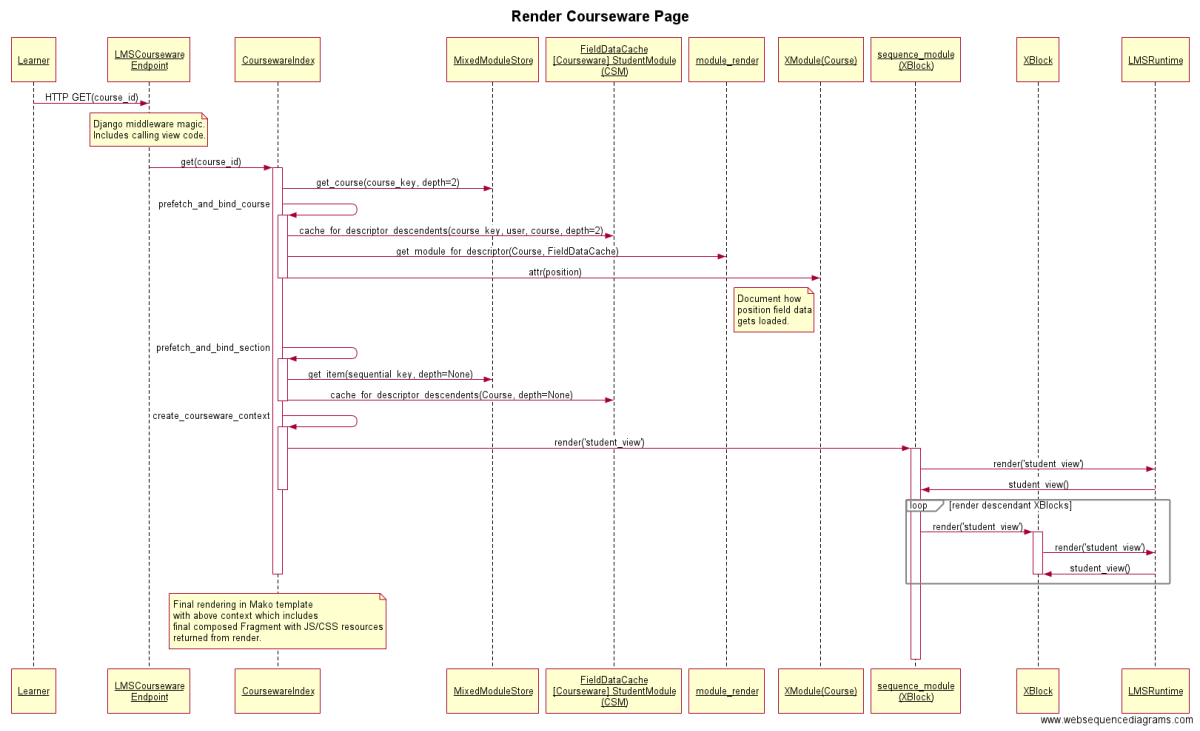
\includegraphics[width=\linewidth]{images/Render_Courseware_Page_Sequence_Diagram.png}
	\caption{Rendering of courseware using XBlocks}
	\label{Fig.1:Sequence diagram}
\end{figure}


\section{Testing and Installing Created XBlock}
\subsection{For Workbench}
We can test a xblock, while running with edX or workbench. We can install the xblock using following
commands and start as a local server, and open the browser to find the link for new xblock
\begin{enumerate}
\item Go to the root directory of new created xblock.
\item Type in the following commands\begin{center}\verb= pip install -e name of xblock=\end{center}
\item run the workbench as a local server using command python manage.py
runserver
\end{enumerate}


\subsection{For Open edX instance}
Clone the repository on our local machine. Testing this first on devstack is always recommended
\begin{enumerate}
\item Enter the shell of your devstack and execute :
\begin{center}\verb= sudo -u edxapp /edx/bin/pip.edxapp install /path/to/cloned/directory=\end{center}
\textbf{Note:} You need to point pip to the directory containing setup.py of our project.\newline For
example: If we cloned this repo in directory called\textbf{ /home/edx/advhtmlxblock} and
\textbf{/home/edx/advhtmlxblock/setup.py}is present then\textbf{ /home/edx/advhtmlxblock} is your
required path
\item (Re)start your LMS and CMS.
\item Login to studio as staff
\item Go to "Advanced Settings" in your course
\item Add word advancedhtml to list of "Advanced Modules"
\item Save changes
\item Advanced HTML component should be present in "Advanced" section in your course.
\end{enumerate}


%%%%%%%%%%%%%%%%%%%%%%%%%%%%%%%%%%%%



\end{document}